\documentclass[a4paper,12pt]{report}
\usepackage[spanish]{babel}
\usepackage[utf8]{inputenc}
\usepackage{graphicx}
\usepackage{url}
%cargamos los paquetes
%fijamos titulo, autor y fecha, creando una página para sólo aparezca el título
\title{Trabajo de técnicas experimentales}
\author{Lorena Díaz Morales\\ Jennifer Cabrera Mesa\\ Claudio García Vargas}
\date{\today}
\begin{document}
\begin{titlepage}
\maketitle 
\end{titlepage}
\tableofcontents
\listoftables
\listoffigures
\chapter{Motivación y objetivos}
\begin{itemize}
 \item
    Objetivo principal : Implementación en python del desarrollo de Taylor
 \item
    Objetivo especifico : Como se comporta la interpolación de una función logaritmica
\end{itemize}
\section{Justificación del trabajo}
Cursando la asignatura de tecnicas experimentales, realizamos este trabajo para aplicar los conocimientos adquiridos
durante el curso sobre python, latex y beamer. Con ello, queremos hacer un estudio sobre la interpolación
de Taylor de una función dada.Veamos las ventajas que tiene este metodo de aproximacion:
\begin{itemize}
 \item 
    La derivacion del polinomio se puede realizar termino a termino lo que hace que resulten operaciones triviales. 
 \item
    Se puede utilizar para calcular valores aproximados de la funcion.
 \item
    Si es posible transformar una funcion mediante el polinomio de Taylor se comprueba que seria la aproximacion optima posible. 
\end{itemize}

Algunas funciones no se pueden escribir como serie de Taylor porque presentan singularidades.Por ejemplo, aquellas funciones que presenten oscilaciones en un intervalo pequeño.
En estos casos se puede conseguir un desarrollo en serie utilizando potencias negativas de x.

  
\section{Objetivos}
\begin{itemize}
 \item 
    Implementación en python para calcular el desarrollo en serie de Taylor para la función f(x)=ln(6x), x $\in$ [1,7]
 \item
    Adquirir práctica a la hora de redactar documentos científicos con latex.
 \item
    Realizar presentaciones con beamer para la exposición en público.
 
\end{itemize}
\chapter{Fundamentos teóricos}
Para este trabajo es necesario presentar los fundamentos que se emplean en la interpolación de Taylor.
Se hará una breve descripción histórica y presentaremos los teoremas y las anotaciones necesarias para el desarrollo del polinomio de Taylor.
\section{Notas históricas sobre el polinomio de Taylor}
Los inicios del polinomio de Taylor se remontan a la época de Zenón de Elea que consideró el problema de sumar una serie infinita para lograr un resultado finito.
Al final dió por imposible este problema pero lo retomaron Demócrito y Arquímedes quedando resuelto el contenido matemático mediante un método exhaustivo.
En el siglo XIV, se dice que los primeros ejemplos del uso de series de Taylor fueron dados por Madhava of Sangamagrama.Tres siglos después, James Gregory publicó varias
series de McLaurin, idea que tomó Taylor perfeccionándola con una formula general para abordar mas casos.

Brook Taylor fue un matemático inglés, nacido en el año 1685, que estudió diversos problemas de las
matemáticas de su época. En su obra Methodus Incrementorum Directa et Inversa, publicada en 1715 ,
desarrollo una nueva parte de la investigación matemática, hoy llamada cálculo de las diferencias finitas.
Entre las distintas aplicaciones, se encontraba el tema de este trabajo, la fórmula del teorema de Taylor.
cuya importancia la descubrió, tiempo después, Lagrange en el año 1772, casi 60 años después de que Taylor
la formulara.
  
Este teorema permite obtener aproximaciones polinómicas de una función en un entorno de un punto en que la función sea diferenciable.
Además el teorema permite acotar el error obtenido mediante dicha estimación.
\section{El polinomio de Taylor}
Si una función f(x) admite derivadas hasta el orden n en a, entonces se puede calcular su 
polinomio de Taylor de grado n centrado en a como se detalla a continuación:
\begin{displaymath}
f(x) = f(a)+f'(a)(x-a) + \frac{f^{(2)}(a)}{2!}(x-a)^2 + \frac{f^{(3)}(a)}{3!}(x-a)^3 + \ldots{} + \frac{f^{(n)}(a)}{n!}(x-a)^n
\end{displaymath}

Expresado como sumatorio, queda de la siguiente forma

\begin{displaymath}
\sum_{n=0}^\infty\frac{f^{(n)}(a)}{n!}(x-a)^{n}
\end{displaymath}

Este polinomio de grado n, se denota $P_n(x;a)$. Es la suma de los n+1 primeros términos de la serie de Taylor.

El teorema de Taylor también se compone de un término llamado resto $R_n(x;a)$, definida por la ecuación

\begin{displaymath}
f(x) = P_n(x;a) + R_n(x;a)
\end{displaymath}

Siendo $R_n(x;a)$

\begin{displaymath}
R_n(x;a) = \frac{1}{n!}\int_{a}^{x} (x-t)^nf^{n+1}(t)dt
\end{displaymath}

Para funciones cuyo comportamiento es bueno, lo esperado es que este término, el resto, tienda a cero cuando n tiende a infinito. En nuestro caso, 
la función se comporta de acuerdo a lo descrito

\begin{displaymath}
R_n(x;a)\rightarrow0 ,n\rightarrow\infty
\end{displaymath}


\chapter{Procedimiento experimental}
\section{Descripción de los experimentos}
Para realizar las pruebas, se han seguido los pasos que se indican a continuación. Se han tomado algunos valores en el intervalo
indicado. Para cada uno de ellos, se han tomado diferentes puntos donde centrar el polinomio y también se ha ido variando el 
grado del polinomio para comprobar en qué medida es mejor el ajuste obtenido, para cada uno de los puntos.

Por otra parte, se ha experimentado, tomando un punto fijo y manteniendo el grado del polinomio, pero variando el lugar de
centralización.
\section{Descripción del material}
Las pruebas de cálculo han sido llevadas a cabo en un ordenador con las siguientes características de hardware y software

\begin{itemize}
 \item Tipo de CPU: Intel(R) Core(TM)2 Duo CPU T5800 @ 2.00GHz
 \item Caché: 2048 KB
 \item Sistema Operativo: Linux
 \item Versión: Linux Mint 14 Nadia
 \item Kernel: 3.5.0-27-generic
 \item Versión de Python: 2.7.3
\end{itemize}

\section{Resultados obtenidos}
Se presentan en las siguientes tablas, los resultados obtenidos.

\begin{table}[htb]
\begin{center}
  \caption{Tabla para x=2}
  \begin{tabular}{|c|c|c|c|c|} %alineación, l=left, c=center, r=right, | separa con línea vertical
  \hline
         Grado  &  Centro  &  Aproximación    &  Valor de f(x)  &  Diferencia        \\ \hline
            3   &   1.75   &  2.46921379883   &  2.48490664979  &  0.0156928509579   \\ \hline
            3   &   1.9    &  2.48240502207   &  2.48490664979  &  0.00250162772088  \\ \hline
            3   &   2.1    &  2.48240514729   &  2.48490664979  &  0.00250150249723  \\ \hline
            3   &   2.25   &  2.46922614378   &  2.48490664979  &  0.0156805060103   \\ \hline
            5   &   1.75   &  2.46915886719   &  2.48490664979  &  0.0157477825985   \\ \hline
            5   &   1.9    &  2.48240352207   &  2.48490664979  &  0.00250312772088  \\ \hline
            5   &   2.1    &  2.48240352209   &  2.48490664979  &  0.00250312749723  \\ \hline
            5   &   2.25   &  2.46915900511   &  2.48490664979  &  0.0157476446822   \\ \hline
            10  &   1.75   &  2.46915829281   &  2.48490664979  &  0.0157483569776   \\ \hline
            10  &   1.9    &  2.48240351957   &  2.48490664979  &  0.00250313021812  \\ \hline
            10  &   2.1    &  2.48240351957   &  2.48490664979  &  0.00250313021812  \\ \hline
            10  &   2.25   &  2.46915829283   &  2.48490664979  &  0.0157483569562   \\ \hline
            15  &   1.75   &  2.46915829282   &  2.48490664979  &  0.0157483569681   \\ \hline
            15  &   1.9    &  2.48240351957   &  2.48490664979  &  0.00250313021812  \\ \hline
            15  &   2.1    &  2.48240351957   &  2.48490664979  &  0.00250313021812  \\ \hline
            15  &   2.25   &  2.46915829282   &  2.48490664979  &  0.0157483569681   \\ \hline
   \end{tabular}
   \label{Tabla}
   \end{center}
\end{table}

\clearpage

\begin{table}[htb]
\begin{center}
  \caption{Tabla para x=3}
  \begin{tabular}{|c|c|c|c|c|} %alineación, l=left, c=center, r=right, | separa con línea vertical
  \hline
         Grado  &  Centro  &  Aproximación    &  Valor de f(x)  &  Diferencia        \\ \hline
            3   &   2.75   &  2.88341439325   &  2.8903717579   &  0.00695736464395  \\ \hline
            3   &   2.9    &  2.88926032968   &  2.8903717579   &  0.00111142821889  \\ \hline
            3   &   3.1    &  2.88926034615   &  2.8903717579   &  0.00111141174491  \\ \hline
            3   &   3.25   &  2.88341600878   &  2.8903717579   &  0.00695574911659  \\ \hline
            5   &   2.75   &  2.88340314068   &  2.8903717579   &  0.00696861721597  \\ \hline
            5   &   2.9    &  2.88926002927   &  2.8903717579   &  0.00111172863041  \\ \hline
            5   &   3.1    &  2.88926002928   &  2.8903717579   &  0.00111172861734  \\ \hline
            5   &   3.25   &  2.8834031487    &  2.8903717579   &  0.00696860919889  \\ \hline
            10  &   2.75   &  2.88340308858   &  2.8903717579   &  0.00696866931621  \\ \hline
            10  &   2.9    &  2.88926002904   &  2.8903717579   &  0.00111172885269  \\ \hline
            10  &   3.1    &  2.88926002904   &  2.8903717579   &  0.00111172885269  \\ \hline
            10  &   3.25   &  2.88340308858   &  2.8903717579   &  0.00696866931596  \\ \hline
            15  &   2.75   &  2.88340308858   &  2.8903717579   &  0.00696866931609  \\ \hline
            15  &   2.9    &  2.88926002904   &  2.8903717579   &  0.00111172885269  \\ \hline
            15  &   3.1    &  2.88926002904   &  2.8903717579   &  0.00111172885269  \\ \hline
            15  &   3.25   &  2.88340308858   &  2.8903717579   &  0.00696866931609  \\ \hline
   \end{tabular}
   \label{Tabla2}
   \end{center}
\end{table}

\clearpage

\begin{table}[htb]
\begin{center}
  \caption{Tabla para x=4}
  \begin{tabular}{|c|c|c|c|c|} %alineación, l=left, c=center, r=right, | separa con línea vertical
  \hline
         Grado  &  Centro  &  Aproximación    &  Valor de f(x)  &  Diferencia         \\ \hline
            3   &   3.75   &  3.17414356442   &  3.17805383035  &  0.00391026592924   \\ \hline
            3   &   3.9    &  3.1774287307    &  3.17805383035  &  0.000625099650957  \\ \hline
            3   &   4.1    &  3.1774287346    &  3.17805383035  &  0.000625095742962  \\ \hline
            3   &   4.25   &  3.17414394696   &  3.17805383035  &  0.0039098833919    \\ \hline
            5   &   3.75   &  3.17413994046   &  3.17805383035  &  0.00391388989164   \\ \hline
            5   &   3.9    &  3.17742863499   &  3.17805383035  &  0.000625195354082  \\ \hline
            5   &   4.1    &  3.17742863500   &  3.17805383035  &  0.000625195352337  \\ \hline
            5   &   4.25   &  3.17413994152   &  3.17805383035  &  0.00391788882403   \\ \hline
            10  &   3.75   &  3.17413993103   &  3.17805383035  &  0.00391389932114   \\ \hline
            10  &   3.9    &  3.17742863495   &  3.17805383035  &  0.000625195393918  \\ \hline
            10  &   4.1    &  3.17742863495   &  3.17805383035  &  0.000625195393919  \\ \hline
            10  &   4.25   &  3.17805383035   &  3.17805383035  &  0.00391389932113   \\ \hline
            15  &   3.75   &  3.17413993103   &  3.17805383035  &  0.00391389932114   \\ \hline
            15  &   3.9    &  3.17742863495   &  3.17805383035  &  0.000625195393918  \\ \hline
            15  &   4.1    &  3.17742863495   &  3.17805383035  &  0.000625195393919  \\ \hline
            15  &   4.25   &  3.17413993103   &  3.17805383035  &  0.00391389932114   \\ \hline
   \end{tabular}
   \label{Tabla3}
   \end{center}
\end{table}

\clearpage

\begin{table}[htb]
\begin{center}
  \caption{Tabla para x=5}
  \begin{tabular}{|c|c|c|c|c|} %alineación, l=left, c=center, r=right, | separa con línea vertical
  \hline
         Grado  &  Centro  &  Aproximación    &  Valor de f(x)  &  Diferencia         \\ \hline
            3   &   4.75   &  3.39869575394   &  3.40119738166  &  0.00250162772088   \\ \hline
            3   &   4.9    &  3.40079734101   &  3.40119738166  &  0.000400040650853  \\ \hline
            3   &   5.1    &  3.40079734229   &  3.40119738166  &  0.000400039370487  \\ \hline
            3   &   5.25   &  3.39869587916   &  3.40119738166  &  0.00250150249724   \\ \hline
            5   &   4.75   &  3.39869425394   &  3.40119738166  &  0.00250312772088   \\ \hline
            5   &   4.9    &  3.40079730165   &  3.40119738166  &  0.000400080010853  \\ \hline
            5   &   5.1    &  3.40079730165   &  3.40119738166  &  0.000400080010487  \\ \hline
            5   &   5.25   &  3.39869425416   &  3.40119738166  &  0.00250312749723   \\ \hline
            10  &   4.75   &  3.39869425144   &  3.40119738166  &  0.00250313021812   \\ \hline
            10  &   4.9    &  3.40079730164   &  3.40119738166  &  0.00040008002134   \\ \hline
            10  &   5.1    &  3.40079730164   &  3.40119738166  &  0.00040008002134   \\ \hline
            10  &   5.25   &  3.39869425144   &  3.40119738166  &  0.00250313021812   \\ \hline
            15  &   4.75   &  3.39869425144   &  3.40119738166  &  0.00250313021812   \\ \hline
            15  &   4.9    &  3.40079730164   &  3.40119738166  &  0.00040008002134   \\ \hline
            15  &   5.1    &  3.40079730164   &  3.40119738166  &  0.00040008002134   \\ \hline
            15  &   5.25   &  3.39869425144   &  3.40119738166  &  0.00250313021812   \\ \hline
   \end{tabular}
   \label{Tabla4}
   \end{center}
\end{table}

\clearpage

\begin{table}[htb]
\begin{center}
  \caption{Tabla para x=6}
  \begin{tabular}{|c|c|c|c|c|} %alineación, l=left, c=center, r=right, | separa con línea vertical
  \hline
         Grado   &  Centro  &  Aproximación    &  Valor de f(x)  &  Diferencia        \\ \hline
            10   &   5      &  3.55534806127   &  3.58351893846  &  0.028170877184    \\ \hline
            10   &   5.1    &  3.56076195126   &  3.58351893846  &  0.0227569871918   \\ \hline
            10   &   5.2    &  3.56558123775   &  3.58351893846  &  0.0179377007058   \\ \hline
            10   &   5.3    &  3.56981434695   &  3.58351893846  &  0.0137045915056   \\ \hline
            10   &   5.4    &  3.5734686026    &  3.58351893846  &  0.0100503358543   \\ \hline
            10   &   5.5    &  3.57655026914   &  3.58351893846  &  0.00696866931621  \\ \hline
            10   &   5.6    &  3.57906458811   &  3.58351893846  &  0.00445435034939  \\ \hline
            10   &   5.7    &  3.58101580824   &  3.58351893846  &  0.00250313021812  \\ \hline
            10   &   5.8    &  3.5824072096    &  3.58351893846  &  0.00111172885269  \\ \hline
            10   &   5.9    &  3.58324112209   &  3.58351893846  &  0.000277816365171 \\ \hline
   \end{tabular}
   \label{Tabla5}
   \end{center}
\end{table}

\clearpage

\begin{figure}[t]
  \begin{center}
    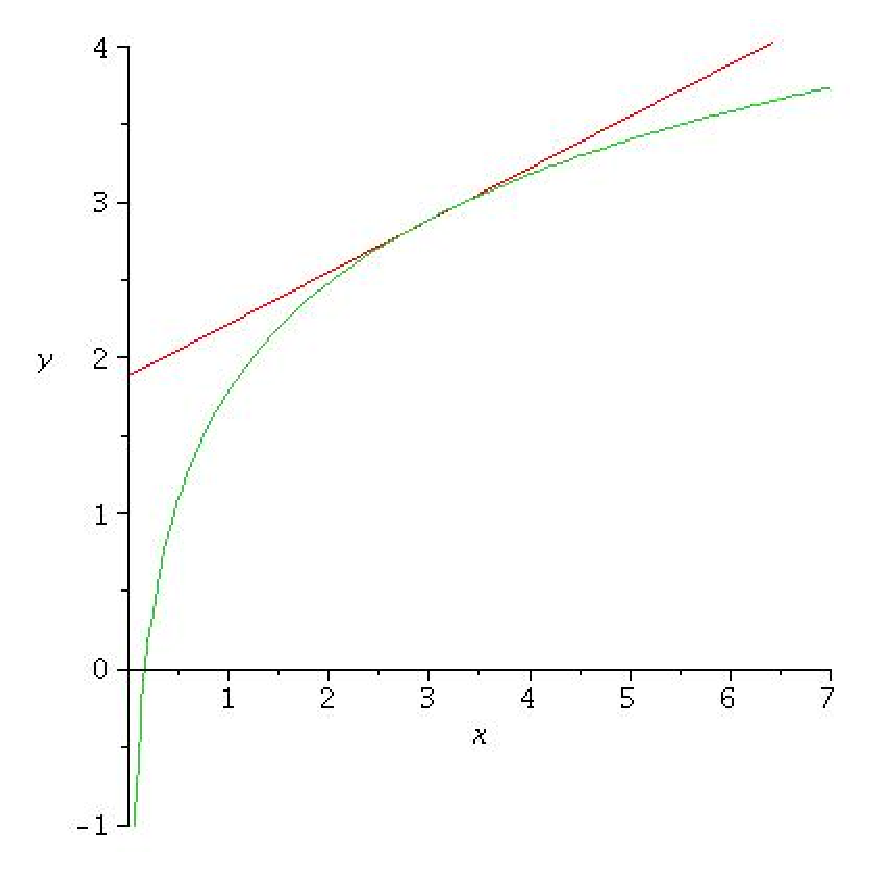
\includegraphics[width=0.5\textwidth]{grafica2.eps}
    \caption{Polinomio de Taylor. Centrado en 6, de grado 2}
    \label{fig:ejemplo}
  \end{center}
\end{figure}

\clearpage

\begin{figure}[t]
  \begin{center}
    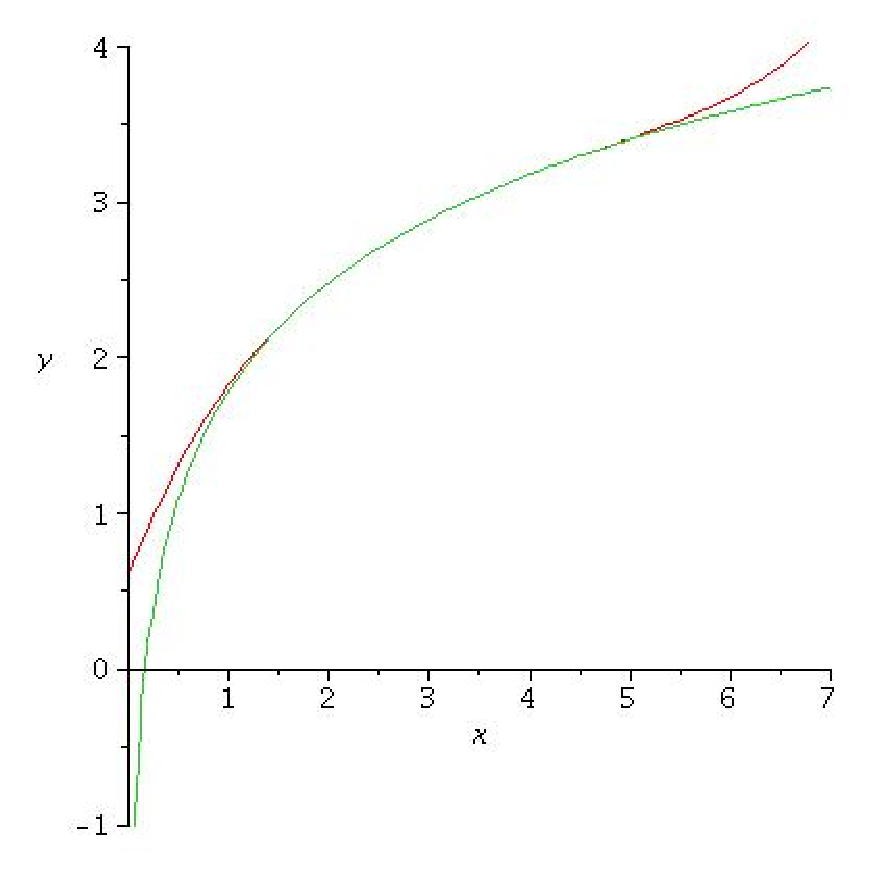
\includegraphics[width=0.5\textwidth]{grafica6.eps}
    \caption{Polinomio de Taylor. Centrado en 6, de grado 6}
    \label{fig:ejemplo2}
  \end{center}
\end{figure}

\clearpage

\begin{figure}[t]
  \begin{center}
    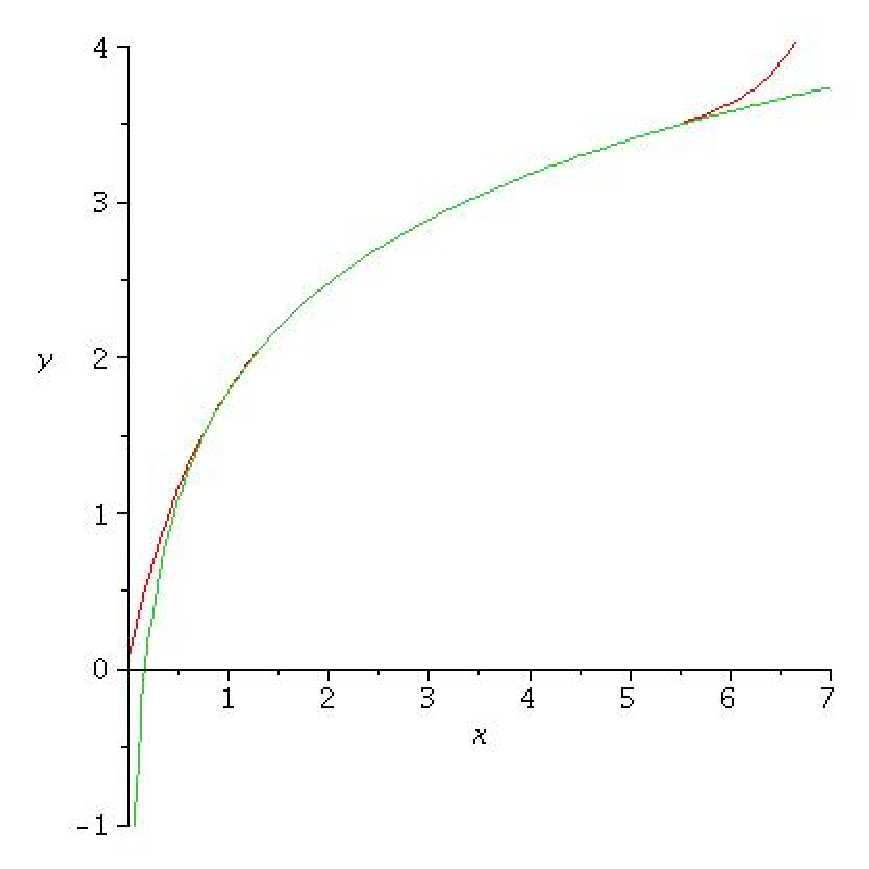
\includegraphics[width=0.5\textwidth]{grafica10.eps}
    \caption{Polinomio de Taylor. Centrado en 6, de grado 10}
    \label{fig:ejemplo3}
  \end{center}
\end{figure}


\clearpage

\section{Análisis de los resultados}

La aproximación de Taylor es de gran importancia para calcular aproximaciones a funciones. Los errores van decreciendo a medida que el grado
del polinomio va aumentando, ya que se incluyen más términos en la suma y aproxima de una manera más cercana si cabe al valor de la función
que queremos hallar en dicho punto.

Otro aspecto a tener muy en cuenta, a la hora de aproximar, es la del centro del polinomio. Esto influye en la calidad de la aproximación, ya
que dependiendo del valor donde se centre, el polinomio tendrá una aproximación deficiente a valores lejanos, porque por muchos términos que 
se introduzcan, no es posible salvar, en general, esa deficiencia. Por contra, si elegimos un centro relativamente cerca del punto a estudiar, 
lo más normal es que se aproxime muy bien al valor original de la función que se está aproximando.

\chapter{Conclusiones}
En esta sección, presentamos las conclusiones finales del trabajo
\begin{itemize}
 \item Las series de Taylor pueden utilizarse para generar esquemas en diferencias finitas. Dichos esquemas se utilizan para aproximar la 
 derivada de una función en un punto donde esté definida la función a estudiar.
 \item Las series de Taylor, dependiendo de la naturaleza de la función, pueden llevar asociados un error, que tenderá a cero si tomamos una
 función lo suficientemente buena como pueden ser: $\sen(x)$, $\cos(x)$, $ln(x)$, \ldots
 \item La aproximación de Taylor se aproxima tanto como queramos, poniendo una mayor cantidad de términos en el polinomio.
 \item Es una herramienta matemática que facilita mucho los cálculos de aproximación de funciones.
 \item Se puede programar rápidamente, ya que no es de gran complejidad. Sólo necesitamos un punto, un lugar donde centrar el polinomio y 
el grado que queremos. Ofrece resultados de manera muy precisa.
\end{itemize}



%creación del apéndice
\appendix
\chapter{Algoritmos}
\section{Interpolador de Taylor}
\begin{verbatim}
#funcion_taylor.py
#!/usr/bin/python

#Autores: Lorena Díaz Morales, Jennifer Cabrera Mesa, Claudio García Vargas

import sys
from math import *

def taylor(x,n,d):                                                                                                        
  subtotal=0                                                                                                              
  tot=0                                                                                                                   
  i=1                                                                                                                     
  while i<=n :                                                                                                            
   ti = ((((-1)**(i+1))*factorial(i-1))/((x**i)*(factorial(i))))*((x-d)**i)                                               
   subtotal = float(subtotal)+float(ti)                                                                                   
   i+=1                                                                                                                   
  valor = float(log(6*d))
  tot = float(valor) + float(subtotal)
  return tot
if __name__=='__main__':
  x = float(sys.argv[1])
  n = int(sys.argv[2])
  d = float(sys.argv[3])
  print ''
  print 'La aproximacion de Taylor es',taylor(x,n,d)
  diferencia=float(float(log(6*x))-float((taylor(x,n,d))))
  l=float(log(6*x))
  print 'La diferencia entre el valor real  interpolacion es',diferencia
  print 'Valor de la funcion orignial en el punto:',l
\end{verbatim}

\begin{thebibliography}{10}
\bibitem{1} 
Larson, Hostetler, Edwards. \emph{Cálculo}. McGraw Hill. 2006. Octava edición.
\bibitem{2}
Sherman K. Stein. \emph{Cálculo y geometría analítica}. McGraw Hill. 1987. Tercera edición.
\bibitem{3}
Tobias Oetiker y otros. \emph{\LaTeXe  en 127 minutos}. Versión 4.20.2, 23 Febrero de 2010
\bibitem{4}
Raúl González Duque. \emph{Python para todos}.
\bibitem{5}
Till Tantau, Josep Wright, Vedran Miletić. \emph{Beamer User Guide}. Versión 3.26, 4 Enero de 2013
\bibitem{6}
\url{www.guiasdeapoyo.net/guias/cuart_mat_e/Serie de Taylor.pdf}
\bibitem{7}
\url{http://www.fceia.unr.edu.ar/lcc/cdrom/Instalaciones/LaTex/latex.html}
\end{thebibliography}

\end{document}
